\documentclass[10pt,a4paper,titlepage]{jreport} % ドキュメントクラスを1つに統一


\usepackage[top=25truemm,bottom=25truemm,left=20truemm,right=20truemm]{geometry} % 余白設定
\usepackage[dvipdfmx]{graphicx} % 画像の挿入
\usepackage{listings} % コードリスト用
\usepackage{jlisting} % 日本語対応のリスト用
\usepackage{float}
\usepackage{jverb} % 日本語のベタ打ち
\usepackage{booktabs}
\usepackage{pgfplots} % グラフ描画用パッケージ
\pgfplotsset{compat=1.18} % バージョン指定

\parindent = 0pt % 段落の字下げを無効化

\usepackage{titlesec}
\usepackage{etoolbox}
\makeatletter
\patchcmd{\chapter}{\if@openleft\cleardoublepage\else\if@openright\cleardoublepage\else\clearpage\fi\fi}{}{}{}
\makeatother
\lstset{breaklines=true, postbreak=\mbox{$\hookrightarrow$}\space, keepspaces=true, escapeinside={\%*}{*)}}

\titleformat{\chapter}[hang] % 章のフォーマットを変更
  {\normalfont\huge\bfseries} % フォント設定
  {\thechapter} % 番号部分の表示形式
  {1em} % 番号とタイトルの間のスペース
  {} % タイトルの前に入れる内容(ここでは空)

\usepackage{amsmath}
\usepackage{xcolor}

\lstset{
  language=Matlab,              % 言語はMATLAB
  basicstyle=\ttfamily,   % フォントは等幅、サイズ小さめ
  keywordstyle=\color{blue},    % キーワード(function, endとか)を青
  commentstyle=\color{green!50!black}, % コメントを深緑
  stringstyle=\color{red!70!black},    % 文字列('...')を赤系
  numbers=left,                 % 行番号を左に表示
  numberstyle=\tiny\color{gray},% 行番号をグレーで小さく
  stepnumber=1,                 % 毎行行番号つける
  numbersep=10pt,               % コードとの間隔
  backgroundcolor=\color{gray!10}, % 背景うっすらグレー
  frame=single,                 % 枠をつける
  rulecolor=\color{black},      % 枠線は黒
  breaklines=true,              % 長い行を折り返す
  breakatwhitespace=false,      % スペースでだけ折り返すか(falseにして自然な折り返し)
  showspaces=false,             % スペースは特別に表示しない
  showstringspaces=false,       % 文字列中のスペースも普通に表示
  tabsize=2                     % タブ幅2
}

\title{知的システム工学実験演習I·II(S101-S102)} % タイトル
\author{
  学生番号:242C2016  氏名:奥村直 \\
  \\
  知的システム工学科システム制御コース
  } % 著者
\date{\today} % 日付
\begin{document}
\setcounter{secnumdepth}{3}
\maketitle

\chapter{制御目的}

 制御目的は2つある。次に簡潔に示す。 \\

1. 倒立状態にある棒が何らかの原因で傾いたとき、台車を動かして、棒を素早く倒立
  状態に戻す。つまり不安定平衡点の安定化である。\\

2. 倒立位置を指定した位置に移動させる。

\chapter{実験装置の概要}

 制御対象として図2(実験マニュアルを参照)に示される倒立振子系を考える。モノレール上に
台車が置かれ、台車上のモノレールと直角な軸に1本の棒(振子)が取り付ける、棒はその
軸まわりに自由に回転できる。台車はベルトとプーリを介して、モータにより駆動され、
モノレール上を走行できる。すなわち、振子は鉛直線とモノレールにより定まる平面に拘束
されて、台車によって動かされるようになっている。\\

 次にこの倒立振子系の制御目的について考える。この倒立振子系は、2つの平衡点をもつ。
1つは棒が鉛直線に沿って垂れ下がった状態が鉛直線に沿って倒立した状態である。前者は
、棒を揺らせば所謂振子になり、揺れは時間が経過により次第に止まるから、安定平衡点
である。後者は、所謂倒立振子であるが、倒立状態にある棒を少しでもつつけば、落ちて
いくから不安点平衡点である。

\chapter{実験結果}

\section{ $M$ と $f$ の測定とシミュレーションによるグラフの出力}

\subsection{状態方程式}

$M$, $f$ を台車の質量と摩擦係数、$m$, $l$, $J$, $c$ は振子の質量、回転軸・重心間距離
、重心まわり慣性モーメント、回転軸摩擦係数、$g$ は重力加速度、$F_H$, $F_V$ は振子が台車
から受ける水平抗力と垂直抗力である。また、$u$ は駆動アンプへの入力電圧、$a$ は駆動アンプ
への入力電圧から台車への駆動力までのゲインである。
実験マニュアルより、図3(実験マニュアルを参照)台車と振子に関する微分方程式が次のように
得られる。

\begin{equation}
M\ddot{r} = au - F_H - f\dot{r}
\end{equation}

\begin{equation}
J\ddot{\theta} = lF_V\sin\theta - lF_H\cos\theta - c\dot{\theta}
\end{equation}

\begin{equation}
m\frac{d^2}{dt^2}(r + l\sin\theta) = F_H
\end{equation}

\begin{equation}
m\frac{d^2}{dt^2}(l\cos\theta) = F_V - mg
\end{equation}

実験マニュアルでは、上記の4式で関係が表されている4つの状態変数からなるベクトルを
状態 $x$ として扱っていた。状態 $x$ を以下に示す。

\begin{equation}
x = 
\begin{pmatrix}
r \\ \theta \\ \dot{r} \\ \dot{\theta}
\end{pmatrix}
\end{equation}

このように定義すると、(3.1)-(3.4)式から、倒立振子系の非線形状態方程式は

\begin{equation}
\dot{x} = f(x,y) = 
\begin{pmatrix}
\dot{r} \\ \dot{\theta} \\ K^-1
\begin{pmatrix}
-f\dot{r} + ml\sin\theta\times\dot{\theta}^2 + au \\ mgl\sin\theta - c\dot{\theta}
\end{pmatrix}
\end{pmatrix}
\end{equation}

よって $K$ は、

\begin{equation}
K = 
\begin{pmatrix}
M+m & ml\cos\theta \\
ml\cos\theta & J + ml^2
\end{pmatrix}
\end{equation}

として得られる。

制御目的より、不安定平衡点 $x = 0$ の近傍の挙動を状態方程式で知ればここでは十分である。
そこで、一次近似された状態方程式を求める。\\

状態方程式は次のように得られる。

\begin{equation}
\dot{x} = Ax + Bu
\end{equation}

ここで、

\[
A =
\begin{pmatrix}
0_2 & I_2 \\
A_21 & A22 \\
\end{pmatrix}
\]

\[
B =
\begin{pmatrix}
0_{2\times1} \\
B_2
\end{pmatrix}
\]

\[
K =
\begin{pmatrix}
M + m & ml \\
ml & J + ml^2 \\
\end{pmatrix}
\]

\subsection{観測方程式}

2つの観測出力を次に示す。

\[
y1 = c_1r
\]

\[
y2 = c_2\theta
\]

ここで、$c_1$ は変位・電圧変換係数、$c_2$ は角度・電圧変換係数である。これらから
なる出力 $y$ を以下に示す

\[
y = 
\begin{pmatrix}
y_1 \\
y_2
\end{pmatrix}
\]

のように定義すると、倒立振子系に対する観測方程式として

\begin{equation}
y = 
\begin{pmatrix}
\begin{pmatrix}
c_1 & 0 \\
0 & c_2 \\
\end{pmatrix} &
0_2
\end{pmatrix}
x
\end{equation}

が得られる。

\subsection{パラメータの同定方法(パラメータ $m$, $f$, $a$)}

本実験では次に示す値を用いて同定した

\begin{table}[htbp]
  \centering
  \caption{パラメータ $m$, $f$, $a$}
  \begin{tabular}{|c|c|}
    \hline
    m & 0.039[kg] \\
    \hline
    l & 0.121[m] \\
    \hline
    a & 0.1[N/V] \\
    \hline
  \end{tabular}
\end{table}

以下に上記に示したパラメータを用いて $M$, $f$ を同定する過程を記述する。

振子を台車から取り外して、台車のステップ応答を測定する。このときの運動方程式は

\begin{equation}
M\ddot{r} = au - f\dot{r}
\end{equation}

である。$u$ から $r$ までの伝達関数 $G$ を求めると

\begin{equation}
G(s) = \frac{K}{s(Ts + 1)}
\end{equation}

となる。ただし、

\begin{equation}
K = \frac{a}{f}
\end{equation}

\begin{equation}
T = \frac{M}{f}
\end{equation}

である。初期状態をゼロとするとき、このシステムのステップ応答は

\begin{equation}
r(t) = KU_0(Te^{\frac{-t}{T}} + t - T)
\end{equation}

である。ただし、$U_0$ はステップの高さである。(3.14)式において $t$ を無限までの
極限とすれば

\begin{equation}
r(t) = KU_0(t - T)
\end{equation}

となり、これから $T$ と $K$ を求め、(3.13)式より $M$ と $f$ を決定することができる。

\subsection{パラメータの同定}

入力電圧を $7V$, $10V$, $14V$ のときで$M$ と $f$をそれぞれ求める。

それぞれのパラメータから得られた実験のグラフを下に示す。

\begin{figure}[H] % Hで「ここに出せ」と指定(\usepackage{here}が必要)
  \centering
  \includegraphics[width=0.6\linewidth]{image1.eps} % 拡張子付きOK(dvipdfmx前提)
\end{figure}

\begin{figure}[H] % Hで「ここに出せ」と指定(\usepackage{here}が必要)
  \centering
  \includegraphics[width=0.6\linewidth]{image2.eps} % 拡張子付きOK(dvipdfmx前提)
\end{figure}

\begin{figure}[H] % Hで「ここに出せ」と指定(\usepackage{here}が必要)
  \centering
  \includegraphics[width=0.6\linewidth]{image3.eps} % 拡張子付きOK(dvipdfmx前提)
\end{figure}

\begin{table}[htbp]
  \centering
  \caption{パラメータ $m$, $f$, $a$}
  \begin{tabular}{|c|c|c|c|}
  \hline
  $U_0[V]$ & 7 & 10 & 14 \\
  \hline
  $K$ & $5.92\times 10^-2$ & $6.19\times 10^-2$ & $5.98\times 10^-2$ \\ 
  \hline
  $T$ & $8.52\times 10^-2$ & $1.22\times 10^-1$ & $7.67\times 10^-2$ \\
  \hline
  $M[kg]$ & $1.44\times 10^-1$ & $1.96\times 10^-1$ & $1.28\times 10^-1$ \\
  \hline
  $f[kg/2]$ & 1.69 & 1.61 & 1.67 \\
  \hline
  \end{tabular}
\end{table}

  $M$, $f$ の値は表3.2に示した通りである。最後に、これらの最確値として平均を
  とると、

\begin{equation}
M = 1.56 \times 10^-1
\end{equation}

\begin{equation}
f = 1.66
\end{equation}

$M$, $f$ の値の決定後のシミュレーションから出力したグラフをいかに示す。

\begin{figure}[H] % Hで「ここに出せ」と指定(\usepackage{here}が必要)
  \centering
  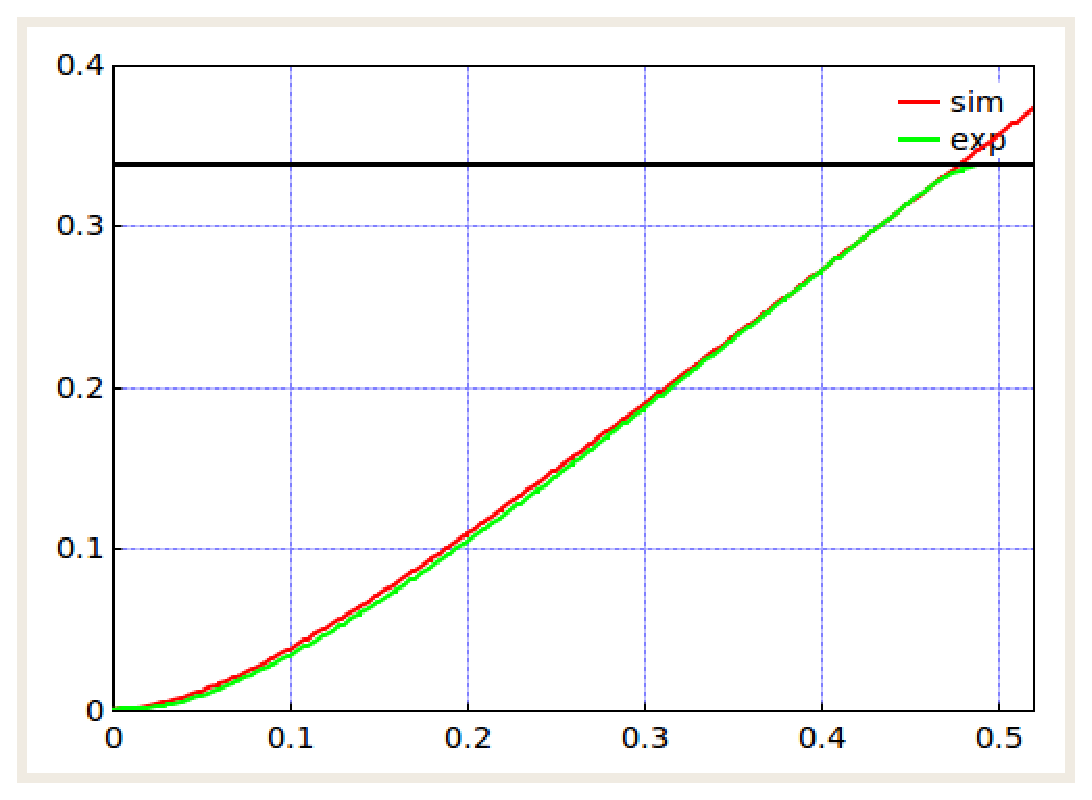
\includegraphics[width=0.6\linewidth]{fMDiff.eps} % 拡張子付きOK(dvipdfmx前提)
\end{figure}

上に示す画像からも分かるように、測定値が理論値と概ね一致しているため $M$, $f$ の決定値は
適切と考えられる。

\section{ $J$ と $c$ の測定とシミュレーションによるグラフの出力}

\subsection{パラメータの同定}

振子を自由振動させることにより,$J$ と $c$ を同定できる。その数式モデルは以下のように表される:

\begin{align}
(J + m\ell^2)\ddot{\theta} &= -mg\ell \sin\theta - c\dot{\theta} \tag{10} \\
y_2 &= c_2 \theta \tag{11}
\end{align}

$\theta$ を微小範囲で考えると,式 (10)-(11) は次のように変形される:

\begin{equation}
\ddot{y}_2 + 2\zeta \omega_n \dot{y}_2 + \omega_n^2 y_2 = 0
\end{equation}

ただし、

\begin{align}
\zeta &= \frac{c}{2\sqrt{mg\ell(J + m\ell^2)}} \\
\omega_n &= \sqrt{\frac{mg\ell}{J + m\ell^2}}
\end{align}

と定義される。

この微分方程式の解は、$0 < \zeta < 1$ のとき、減衰振動となり次のように表される:

\begin{equation}
y_2(t) = y_2(0)\sqrt{1 - \zeta^2} \cdot \exp(-\omega_n \zeta t) \cdot \sin\left( \omega_n \sqrt{1 - \zeta^2} t + \phi \right)
\end{equation}

ただし、

\begin{equation}
\phi = \tan^{-1} \left( \frac{\sqrt{1 - \zeta^2}}{\zeta} \right)
\end{equation}

この $\lambda$ は **対数減衰比**と呼ばれる。また、

\begin{equation}
T_2 = \frac{2\pi}{\omega_n \sqrt{1 - \zeta^2}} \tag{13}
\end{equation}

が成り立つ。

したがって、$J$ と $c$ は次のように与えられる:

\begin{align}
J &= \frac{mg\ell T_2^2}{4\pi^2 + \lambda^2} - m\ell^2 \\
c &= \frac{2\lambda(J + m\ell^2)}{T_2} \tag{14}
\end{align}

与式より、$J$ と $c$ は次のように測定され、定まった。

\begin{equation}
J = 4.20 \times 10^-4
\end{equation}

\begin{equation}
c = 8.49 \times 10^-5
\end{equation}


次にこのときに出力されたグラフを掲載する。

\begin{figure}[H] % Hで「ここに出せ」と指定(\usepackage{here}が必要)
  \centering
  \includegraphics[width=0.6\linewidth]{image4.eps} % 拡張子付きOK(dvipdfmx前提)
\end{figure}


\section{台車振子系の安定性と可制御性判定の結果}


倒立振子の状態方程式は以下のように与えられる:

\begin{equation}
\dot{x} = A x + B u
\end{equation}

ここで $u$ は駆動アンプへの入力電圧、$x$ は状態変数ベクトルであり、

\begin{equation}
x = \begin{pmatrix}
r \\
\theta \\
\dot{r} \\
\dot{\theta}
\end{pmatrix}
\end{equation}

と定義される。

行列 $A$, $B$ は以下のように表される:

\begin{align}
A &= \begin{bmatrix}
O_2 & I_2 \\
A_{21} & A_{22}
\end{bmatrix}, \quad
B = \begin{bmatrix}
O_{2 \times 1} \\
B_2
\end{bmatrix}
\end{align}

ここで、
\begin{align*}
I_2 &= \text{2次の単位行列}, \quad
O_2 = \text{2次の零行列}, \quad
O_{2 \times 1} = \text{2×1 の零行列}, \\
K &= \begin{bmatrix}
M + m & m\ell \\
m\ell & J + m\ell^2
\end{bmatrix}, \\
A_{21} &= K^{-1} \begin{bmatrix}
0 & 0 \\
0 & mg\ell
\end{bmatrix}, \quad
A_{22} = K^{-1} \begin{bmatrix}
-f & 0 \\
0 & c
\end{bmatrix}, \quad
B_2 = K^{-1} \begin{bmatrix}
a \\
0
\end{bmatrix}
\end{align*}

\subsection*{安定性判定}

この系が安定であるためには、行列 $A$ の固有値のすべての実部が負である必要がある。  
図5に示すように、行列 $A$ の固有値はすべて実部が負であり、この系は安定であることが確認できた。

\section{制御器設計時のシミュレーション}

二次形式評価関数は以下のように定義される:

\begin{equation}
J = \int_0^{\infty} \left( \frac{q_1}{2} r^2 + \frac{q_2}{2} \theta^2 + \frac{q_3}{2} \dot{r}^2 + \frac{q_4}{2} \dot{\theta}^2 \right) dt
\end{equation}

ここで、$q_1$, $q_2$, $q_3$, $q_4$ はそれぞれ台車位置 $r$、振子角度 $\theta$、台車速度 $\dot{r}$、振子角速度 $\dot{\theta}$ に対応する重み係数であり、各状態の重要度を調整するために用いられる。

システムの安定化を目的として、状態フィードバックによる行列 $A$ の固有値を求め、特に以下の2つの固有値に着目する:

\begin{itemize}
  \item 第1行第1列の固有値(台車位置に対応)
  \item 第2行第1列の固有値(振子角度に対応)
\end{itemize}

これらの固有値の実部を大きく負にするように、重み係数を変えてシミュレーションを行った。

\subsection{q1のとき}

\[
\begin{bmatrix}
-0.0598141 + 0i \\
-1.53685 + 0i \\
-15.4365 + 10.6284i \\
-15.4365 - 10.6284i \\
\end{bmatrix}
\]

\subsubsection{q1の画像}

\begin{figure}[H] % Hで「ここに出せ」と指定(\usepackage{here}が必要)
  \centering
  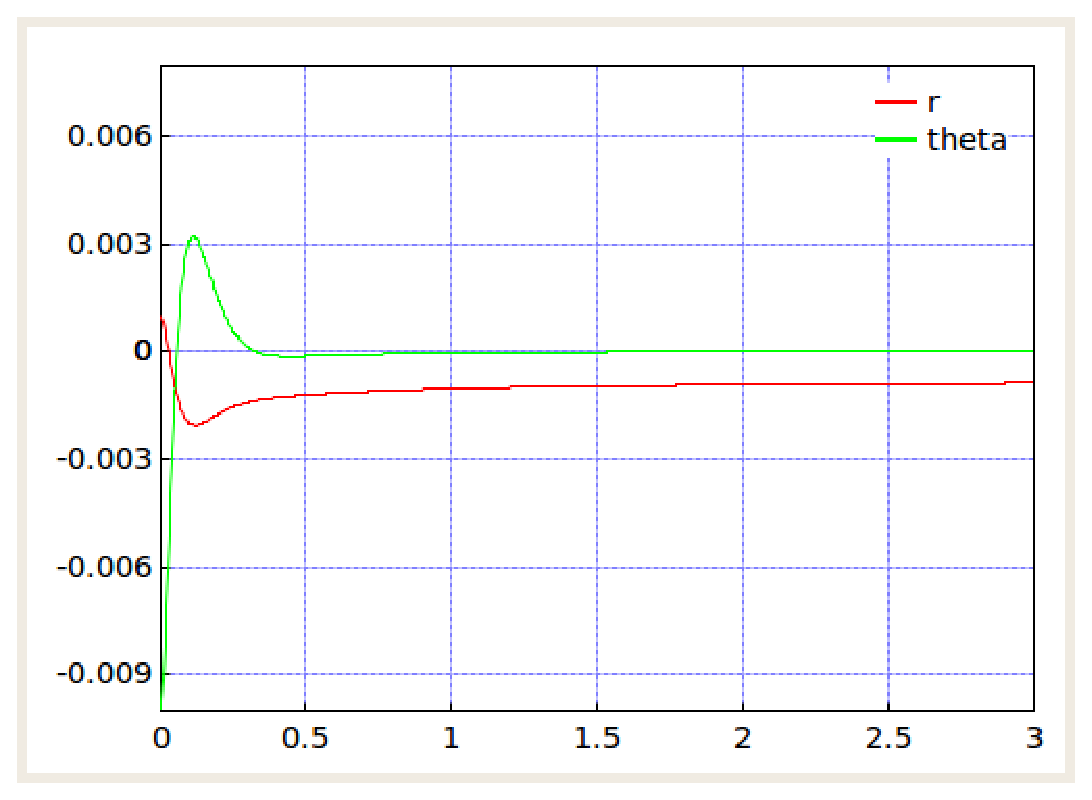
\includegraphics[width=0.6\linewidth]{0400Src.eps} % 拡張子付きOK(dvipdfmx前提)
\end{figure}

\subsection{q2のとき}

\[
\begin{bmatrix}
-5.90179 + 0i \\
-6.38572 + 2.13196i \\
-6.38572 - 2.13196i \\
-12.0712 + 0i \\
\end{bmatrix}
\]

\subsubsection{q2の画像}

\begin{figure}[H] % Hで「ここに出せ」と指定(\usepackage{here}が必要)
  \centering
  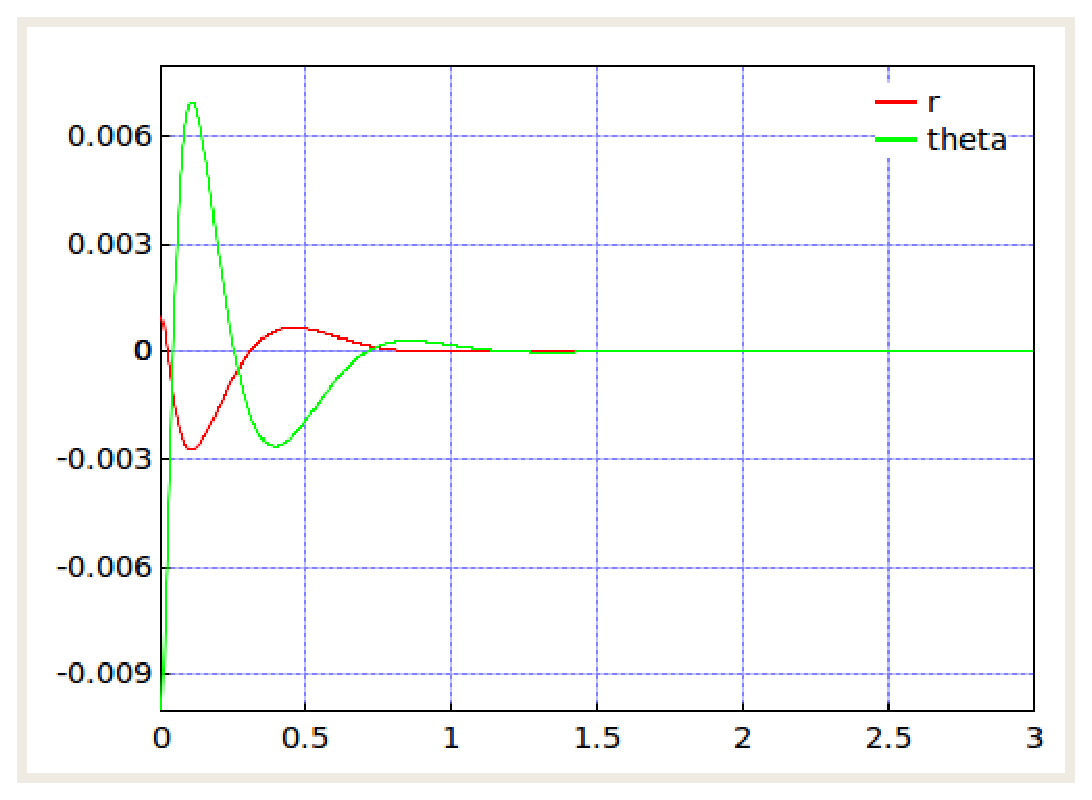
\includegraphics[width=0.6\linewidth]{4000Src.eps} % 拡張子付きOK(dvipdfmx前提)
\end{figure}

\section{倒立実験のグラフ}

\begin{figure}[H] % Hで「ここに出せ」と指定(\usepackage{here}が必要)
  \centering
  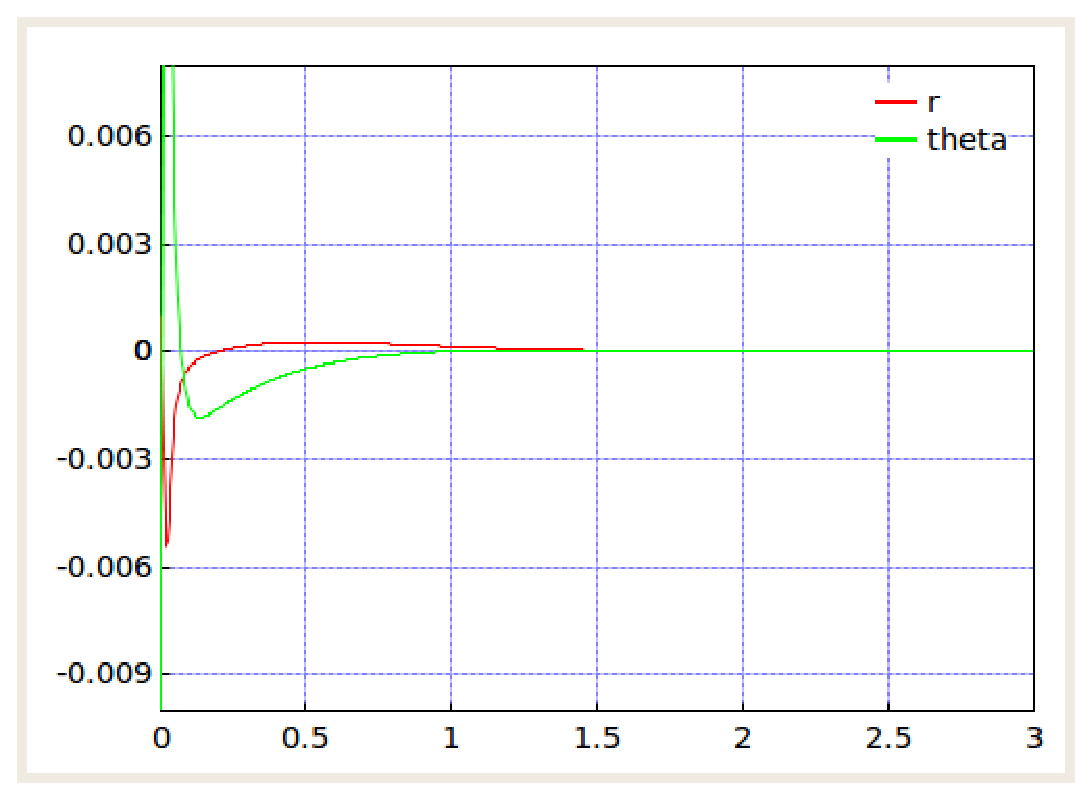
\includegraphics[width=0.6\linewidth]{7700Src.eps} % 拡張子付きOK(dvipdfmx前提)
\end{figure}

\begin{figure}[H] % Hで「ここに出せ」と指定(\usepackage{here}が必要)
  \centering
  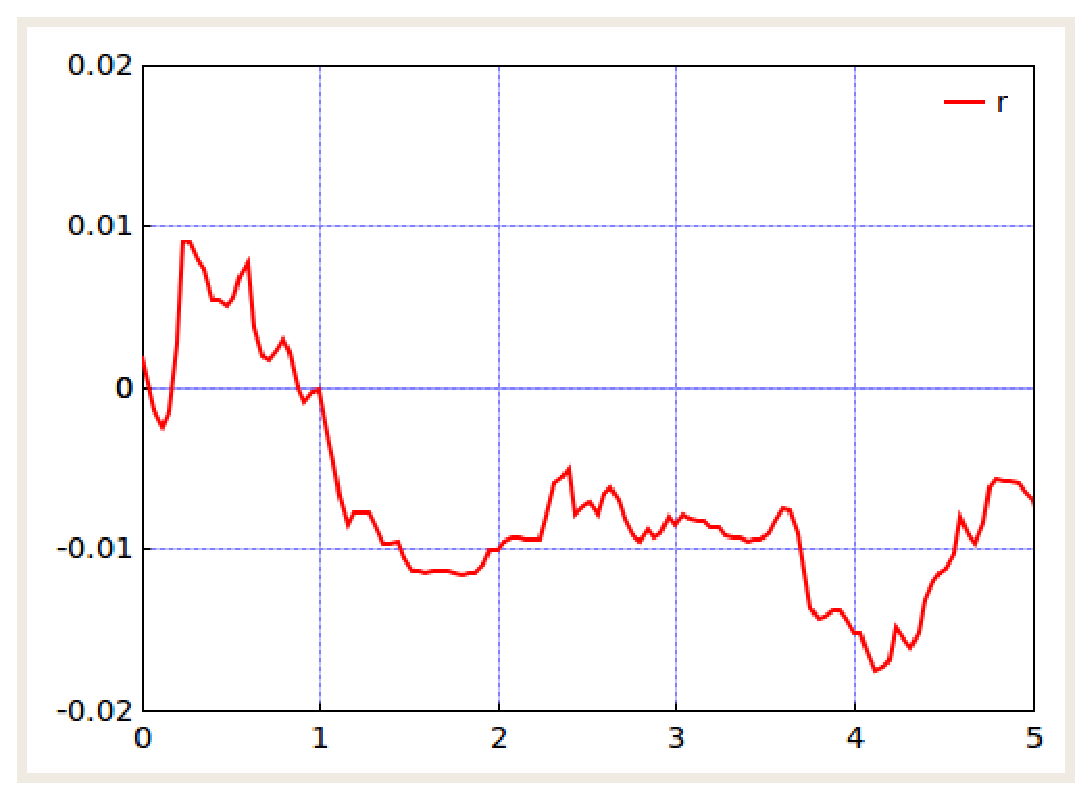
\includegraphics[width=0.6\linewidth]{7700rSrc.eps} % 拡張子付きOK(dvipdfmx前提)
\end{figure}

\begin{figure}[H] % Hで「ここに出せ」と指定(\usepackage{here}が必要)
  \centering
  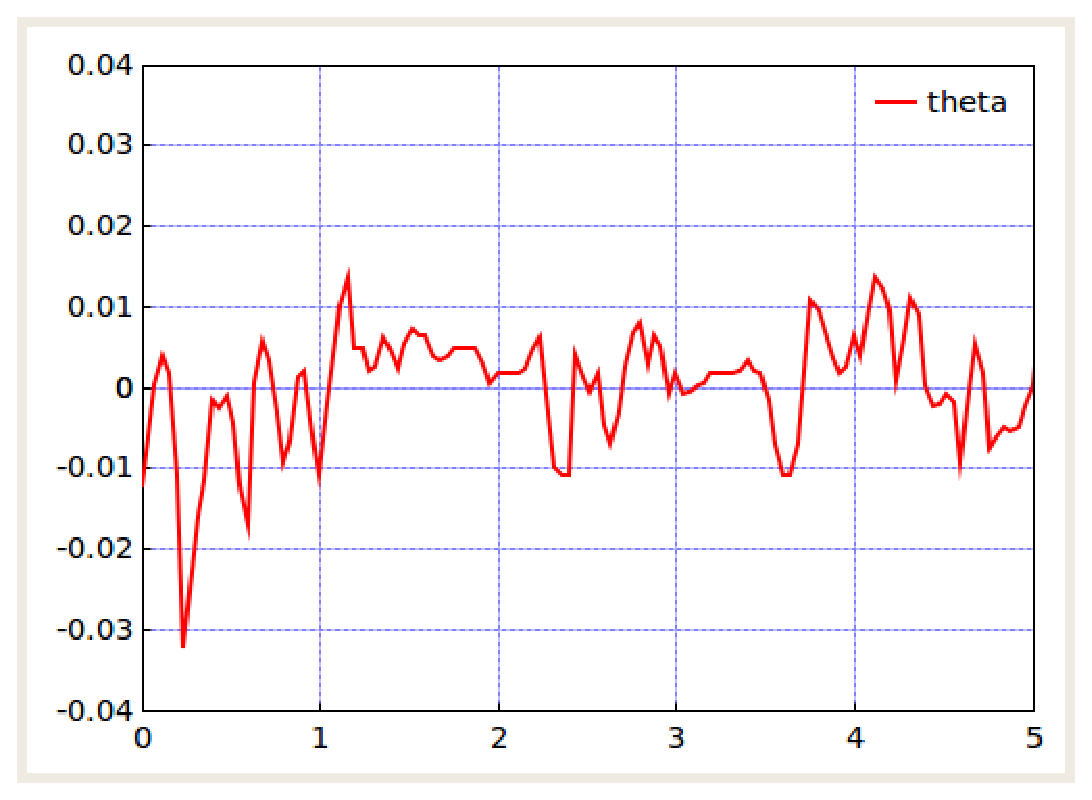
\includegraphics[width=0.6\linewidth]{7700thSrc.eps} % 拡張子付きOK(dvipdfmx前提)
\end{figure}

\begin{figure}[H] % Hで「ここに出せ」と指定(\usepackage{here}が必要)
  \centering
  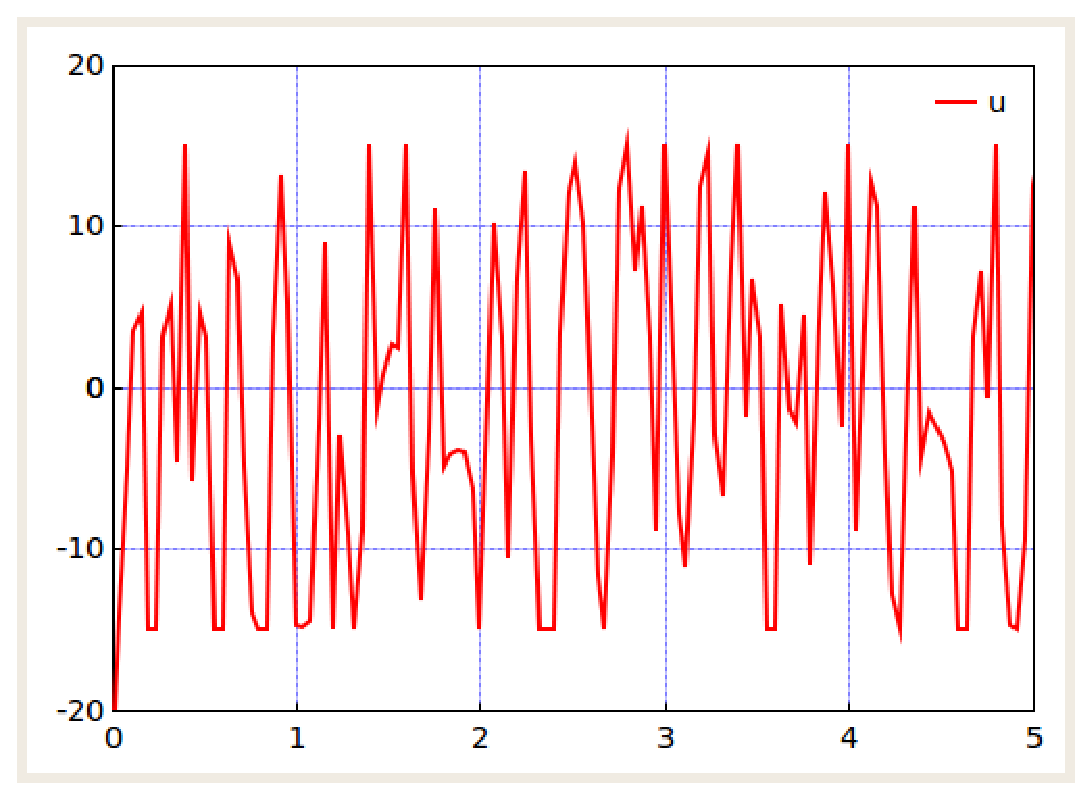
\includegraphics[width=0.6\linewidth]{7700uSrc.eps} % 拡張子付きOK(dvipdfmx前提)
\end{figure}

\chapter{課題}

\section{課題1}

アニメーションにおいては、振子を回転させるといった制御を行ったが、これは実際の実験で行う場合には危険を伴う可能性がある。
回転運動は、振子を倒立させるよりも大きな力が左右に加わるため、万が一振子が人に接触した場合、重大な事故につな
がるおそれがある。また、振子の長さを伸ばして運動を行わせた場合には、モデルとの誤差や予期せぬ外乱により想定外の運動を
生じる可能性があり、安全面のリスクが高まると考える。

\section{課題2}

システム制御における「モデル」とは、制御対象を状態方程式や観測方程式などの数式により記述したものであり、制御設計や
シミュレーションを行う上での基盤となる。一方、計算機は、そのモデルに基づいて特性解析(制御可能性・安定性の
評価など)を行ったり、制御目的を達成するために設計された制御器により、実際にシステムが適切に動作するかをシミュレーションする役割を担っている。すなわち、モデルと計算機は、制御設計とその検証を進める上で不可欠な要素である

\chapter{参考文献}

知的システム工学実験演習 I·II(S101-S102)
–モデルに基づく制御設計とシミュレーション– 

\end{document}